%%This is a very basic article template.
%%There is just one section and two subsections.
\documentclass[10pt,conference]{IEEEtran}

%to handle ranges of citations in IEEEtran
\usepackage[noadjust]{cite}
\renewcommand{\citepunct}{,\penalty\citepunctpenalty\,}
\renewcommand{\citedash}{--}% optionally

%To fix ``fi'' encoding
\usepackage{cmap}
\usepackage{amsthm}
\usepackage{amsmath}
\usepackage{listings}
\usepackage{amsfonts}
\usepackage{graphicx}
\usepackage{courier}
\usepackage{algorithm}
\usepackage[noend]{algpseudocode}
%--- Return lines start in a new line
\let\oldReturn\Return
\renewcommand{\Return}{\State\oldReturn}
%---
\usepackage[table,xcdraw]{xcolor}
\usepackage{float}
\usepackage{hyperref}
\usepackage{mathtools}
\usepackage[framemethod=TikZ]{mdframed}
\usepackage[]{inputenc}
\usepackage[T1]{fontenc}
\usepackage{placeins}
\usepackage{amsmath,amssymb}
\usepackage{xspace}
\usepackage[font=footnotesize]{caption}
\captionsetup[table]{skip=10pt}
%to solve the hyperref problem of jumping to wrong places
%\usepackage[all]{hypcap}
\usepackage[framemethod=TikZ]{mdframed}
\usepackage{booktabs}
\usepackage{fancyvrb}
\usepackage{relsize}
\graphicspath{{images/}}
%\usepackage[ruled,shortend,linesnumbered,algo2e]{algorithm2e}  % algo2e = use
% \begin{algorithm2e}
\usepackage{float}
\usepackage{subfig}
\usepackage{framed}

\newtheorem{theorem}{Theorem}
\newtheorem{lemma}{Lemma}
\newtheorem{corollary}{Corollary}

\newcommand{\aeval}{\textsc{AE-VAL}\xspace}
\newcommand{\jkind}{\textsc{JKind}\xspace}

\newcommand{\jsyn}{\textsc{JSyn}\xspace}
\newcommand{\jsynvg}{\textsc{JSyn-vg}\xspace}
\newcommand{\smtlibtoc}{\textsc{SMTLib2C}\xspace}
\newcommand{\lustrev}{\textsc{LustreV6}\xspace}

\newcommand{\isSat}{\textsc{isSat}\xspace}
\newcommand{\isUnSat}{\textsc{isUnsat}\xspace}

\newcommand{\viable}{{\mathsf {Viable}}}
\newcommand{\reachable}{{\mathsf {Reachable}}}

\newcommand{\extend}{{\mathsf {Extend}}}
\newcommand{\basecheck}{{\mathsf {BaseCheck}}}
\newcommand{\extendcheck}{{\mathsf {ExtendCheck}}}

\newcommand{\glb}{\textit {GLB}\xspace}
\newcommand{\lub}{\textit {LUB}\xspace}
\newcommand{\tuple}[1]{\langle #1 \rangle}

\renewcommand{\labelitemi}{\tiny$\blacksquare$}

\newcommand{\andreas}[1]{\textcolor{blue}{Andreas: #1}}
\newcommand{\mike}[1]{\textcolor{red}{Mike: #1}}
\newcommand{\andrew}[1]{\textcolor{green}{Andrew: #1}}
\newcommand{\john}[1]{\textcolor{orange}{John: #1}}
\newcommand{\grigory}[1]{\textcolor{brown}{Grigory: #1}}
\newcommand{\arie}[1]{\textcolor{purple}{[Arie: #1]}}
\newcommand{\huajun}[1]{\textcolor{yellow}{[Huajun: #1]}}

\newcommand{\realizable}{\textsc{realizable}}
\newcommand{\unrealizable}{\textsc{unrealizable}}
\newcommand{\skolems}{\textit{Skolem}}
\newcommand{\aevalres}{\textit{aevalResult}}
\newcommand{\init}{\textit{init}}
\newcommand{\subs}{\textit{validRegion}}
\newcommand{\isValid}{\textsc{isValid}\xspace}
\newcommand{\isInvalid}{\textsc{isInvalid}\xspace}
%\newcommand{\isSat}{\textsc{isSat}\xspace}
\newcommand{\isUnsat}{\textsc{isUnsat}\xspace}

\newcommand\eqdef{\mathrel{\stackrel{\makebox[0pt]{\mbox{\normalfont\tiny def}}}{=}}}

\newcounter{template}
\newenvironment{template}[1][htb]
  {
   \begin{algorithm2e}[#1]%
   \SetAlgorithmName{Template}
  }{\end{algorithm2e}}

\newenvironment{requirement}
{\vspace{0.05in}
 \begin{mdframed}[roundcorner=10pt,backgroundcolor=gray!20]}
{\end{mdframed}}



\begin{document}
\title{Validity Guided Synthesis of Reactive Systems from Assume-Guarantee Contracts}

\author{\IEEEauthorblockN{Andreas Katis\IEEEauthorrefmark{1}, Grigory Fedyukovich\IEEEauthorrefmark{2}, Andrew Gacek\IEEEauthorrefmark{3}\\ John
Backes\IEEEauthorrefmark{3}, Arie Gurfinkel\IEEEauthorrefmark{4}, Huajun
Guo\IEEEauthorrefmark{1} and
Michael W. Whalen\IEEEauthorrefmark{1}}
\IEEEauthorblockA{\IEEEauthorrefmark{1}Department of Computer Science and
Engineering,
University of Minnesota\\
Email: \{katis001,guoxx663\}@umn.edu, whalen@cs.umn.edu}
\IEEEauthorblockA{\IEEEauthorrefmark{2}University of Washington Paul G. Allen School of Computer Science \& Engineering\\
Email: grigory@cs.washington.edu}
\IEEEauthorblockA{\IEEEauthorrefmark{3}Rockwell Collins Advanced Technology Center\\
Email: \{andrew.gacek,john.backes\}@rockwellcollins.com}
\IEEEauthorblockA{\IEEEauthorrefmark{4}Department of Electrical and Computer
Engineering, University of Waterloo\\
Email: agurfinkel@uwaterloo.ca}}
\maketitle

\begin{abstract}

%shortened version due to 200 word limit
Automated synthesis of reactive systems using only
specification knowledge is a popular and well
explored subject in formal verification. \andrew{The following
  sentance is hard to read and I don't know what it means enough to
  fix it.}
A variety of approaches
have been proposed in the recent years, through inductive
and functional synthesis, while template-based, counterexample-guided and predicate abstraction techniques have proved
useful towards extending the applicability of such algorithms
to solving difficult problems. In this paper, we propose a novel
approach to program synthesis, which is based on the validity
of a $\forall\exists$-formula. The approach is inspired from verification
techniques that construct inductive invariants, like Property
Directed Reachability, and is completely automated. The original
problem space is recursively refined by blocking out regions of
unsafe states, with the goal being the discovery of a fixpont that
describes safe reactions. If such a fixpoint
is found, we construct a witness that is directly translated into an implementation. We implemented the algorithm in the \jkind model checker, and exercised it against contracts written using
the Lustre specification language. Experimental results show
how the new algorithm yields better performance as well as
soundness for ``unrealizable'' results when compared to \jkind's
existing synthesis procedure, an approach based on the construction of k-inductive proofs of realizability.


\iffalse
Automated synthesis of reactive systems using only specification knowledge is one of
the most popular and well explored subjects in formal verification. A variety of
approaches have been proposed in the recent years, through inductive and
functional synthesis, while template-based, counterexample-guided and predicate abstraction techniques
have been proved useful towards extending the applicability of such algorithms
to solving difficult problems. In this paper, we propose a novel approach to
program synthesis, which is based on the validity of a $\forall\exists$-formula.
The approach is inspired from verification techniques that construct
inductive invariants, like Property Directed Reachability, and is completely automated. The original
problem space is recursively refined by blocking out regions of unsafe states, with the goal being the discovery of a
fixpont that describes a region containing safe reactions. If such a fixpoint
is found, we construct a witness that can be directly transformed into an
implementation using mainstream programming languages, like C. We implemented
the algorithm in the \jkind model checker, and exercised it against contracts
written using the Lustre specification language. Experimental results show how
the new algorithm yields better performance as well as soundness for ``unrealizable'' results when compared to \jkind's existing synthesis procedure, an approach that is based on the construction of k-inductive proofs of realizability.
\fi
\end{abstract}


\section{Introduction}

Program synthesis is one of the most challenging problems in the area of formal verification. The objective is to describe an efficient process to automatically derive implementations that are guaranteed to comply with specifications expressed in the form of logic formulas. This area of research owes its origins to Church~\cite{church1962logic} (otherwise known as Church's Problem), and ever since it was first expressed, has enjoyed a considerable amount of contributions.

The first important attempt to synthesize reactive systems came from Pnueli and Rosner~\cite{pnueli1989synthesis}, but the problem has seen an increased popularity in the more recent years, mostly due to the huge impact from work on Satisfiability Modulo Theories~\cite{BarFT-SMTLIB} (SMT). As a result, the problem has been well explained for the area of propositional specifications~\cite{gulwani2010dimensions}, and a great number of approaches have surfaced to tackle the challenge from different perspectives. Template-based techniques~\cite{srivastava2013template}, focus on synthesizing programs that
match a certain shape (the template) while {\em inductive synthesis} uses the idea of refining the problem space using counterexamples, in order to converge to a solution~\cite{flener2001inductive}. A different category is that of \textit{Functional synthesis}, in which the goal is to fill in ``gaps'' in an already existing implementation, with synthesized code~\cite{kuncak2013functional}.

In this work, we describe a novel approach that can effectively synthesize
programs using specifications written in the form of an arbitrary {\em
assume/guarantee contract}. The technique has been exercised on specifications
of safety properties in linear real and integer arithmetic (LIRA),
but it remains generic enough to be extended to other theories
in the future. This is a ``hands-off'' approach, as there is no
requirement from the user to interact with the underlying machinery,
\andreas{I edited the way multiple citations look (all in one pair of
brackets). I'm not sure if this is allowed, so please change it if you know.}
unlike~\cite{ryzhyk2014user,ryzhyk2016developing}, and is capable of providing solutions without the guidance of templates, like
in~\cite{beyene2014constraint}.

The main idea of the algorithm was inspired by the IC3 algorithm, its
technique otherwise known as Property Directed Reachability
(PDR)~\cite{bradley2011sat,een2011efficient}. In PDR, the goal is to discover an
inductive invariant for a property, by recursively blocking generalized regions describing unsafe states. In a similar concept, we attempt
to reach a greatest fixpoint that contains states usable indefinitely by the
system, in order to react to unpredictable environment behaviour, while
complying to well-defined specification. As such, beginning from the entire
problem space, we recursively block regions of states that violate the contract, using \textit{regions of validity} that are
generated by non-valid $\forall\exists$-formulas. If the refined
$\forall\exists$-formula is valid, we reach an approximation of a fixpoint which can effectively be used by the specified transition relation, to
provide safe reactions to environment inputs.\john{This is a little bit confusing to me. It sounds like we use a ``approximation of the fixpoint'' to synthesis the implementation. This approximation is continually refined until we indeed reach a ``true fixpoint'' that we use to derive the implementation. Correct?"} We then extract a witness for the
formula's satisfiability, which can be directly transformed into the
language intended for the system's implementation.

The algorithm was implemented as a feature in the \jkind model checker, which
already had unofficial support for program synthesis according to work from
Katis~\textit{et al.} based on k-inductive proofs of a contract's
realizability~\cite{gacek2015towards,katis2016towards,katis2016synthesis}.
Our approach does not depend on k-induction, but is still based on the general
concept of extracting a witness that satisfies a $\forall\exists$-formula, using
the \aeval Skolemizer~\cite{fedyukovich2015automated}. To extract such a witness, we do not depend on a k-inductive proof, but instead use the \textit{regions of validity} that \aeval can generate from non-valid formulas,
to reach a fixpoint of satisfiable assignments to state variables.
This approach is a direct improvement over the k-inductive method in two
important aspects: performance, and soundness of `unrealizable' results. While
the former is self-explanatory, with the latter we refer to cases where the
k-inductive algorithm would spuriously report a contract as `unrealizable', when a correct
implementation actually exists. This unsoundness stems from the pessimistic
behavior of the k-inductive algorithm, as it is not capable of
considering only a
``safe'' subset of the state space. We were able to confirm our claims
by comparing the two algorithms under a comprehensive benchmark suite containing
contracts that were initially used in verification problems, as well as
specification for industrial-level designs.

Section~\ref{sec:example} briefly describes the Cinderella-Stepmother problem that we will be using as an example throughout the paper. In Section~\ref{sec:background} we provide the necessary formal and semantics background. Section~\ref{sec:synthesis} we present the validity-guided approach to synthesizing implementations. 
An outline of the algorithm's implementation is described in Section~\ref{sec:impl}. Section~\ref{sec:results} depicts the advancements of our validity-guided
approach, comparing it against a method based on k-induction that exists under the same framework. We discuss the differences of our work with closely related ideas in Section~\ref{sec:related} and we conclude by providing potential directions for future work in Section~\ref{sec:conclusion}.

	
%%% Local Variables:
%%% TeX-master: "document"
%%% End:

\section{Overview: The Cinderella-Stepmother Game}
\label{sec:example}

We illustrate the flow of the validity guided-synthesis algorithm using a variation of the minimum-backlog
problem, the two player game between Cinderella and her wicked Stepmother, first expressed by Bodlaender \textit{et al.}~\cite{bodlaender2012cinderella}.

The main objective for Cinderella (i.e. the reactive system) is to prevent a
collection of buckets from overflowing with water. On the other hand,
Cinderella's Stepmother (i.e. the system's environment) refills the buckets with a predefined amount of water that is distributed in a random fashion between the buckets.
For the running example, we chose an instance of the game that has been
previously used in template-based synthesis~\cite{beyene2014constraint}. In this instance, the game is described
using five buckets, where each bucket can contain up to two units of water.
Cinderella has the option to empty two adjacent buckets at each of her turns,
while the Stepmother distributes one unit of water over all five buckets. In the context of this paper we use this example to show how specification is expressed, as well as how we can synthesize an efficient implementation that describes reactions for Cinderella, such that a bucket overflow is always prevented.

\begin{figure}[!t]
\centering
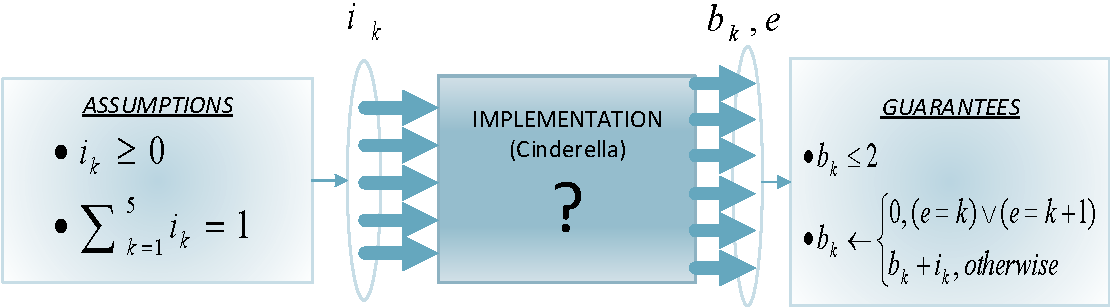
\includegraphics[scale=0.55]{agcontracttilted-crop.pdf}
\caption{An Assume-Guarantee Contract.}
\label{fg:agcontract}
\end{figure}

We represent the system requirements using an \textit{Assume-Guarantee
Contract}. The \emph{assumptions} of the contract restrict the possible inputs that the
environment can provide to the system, while the \emph{guarantees}
describe safe reactions of the system to the outside world.

A (conceptually) simple example is shown in Fig.~\ref{fg:agcontract}. The contract describes a possible set of requirements for a specific instance of the Cinderella-Stepmother game. % that we introduced in Sect.~\ref{sec:example}.
Our goal is to synthesize an implementation that describes Cinderella's winning region of the game. Cinderella in this case is the implementation, as shown by the middle box in Fig.~\ref{fg:agcontract}. Cinderella's inputs are five different values $i_k$, $1 \leq k \leq 5$, determined by a random distribution of one unit of water by the Stepmother. During each of her turns Cinderella has to make a choice denoted by the output variable $e$, such that the buckets $b_k$ do not overflow during the next action of her Stepmother. We define the contract using the set of assumptions $A = \{i_k \geq 0, \sum_{k=1}^{5} i_k = 1\}$ and the guarantees $G = \{b_k \leq 2, b_k = ite((e=k \lor e=k+1), 0, (b_k+i_k))\}$. For the particular example, it is possible to construct at least one implementation that satisfies the guarantee constraints, given the input assumptions. The proof of existence of such an implementation is the main concept behind the \emph{realizability} problem, while the automated construction of a witness implementation is the main focus of \emph{program synthesis}.


Since the contract in Fig.~\ref{fg:agcontract} is \emph{realizable}, there should exist at least one implementation, and we
are seeking for an efficient synthesis procedure that could provide it.
On the other hand, consider a variation of the example, where $A = \varnothing$. This is a practical case of an
\emph{unrealizable} contract, as there is no feasible Cinderella implementation that can correctly react to Stepmother's actions. An example counterexample allows the Stepmother to pour random amounts of water into the buckets, leading to overflow of at least one bucket during each of her turns.

\section{Background}
\label{sec:background}
%\label{sec:formals}
We use two disjoint sets, $state$ and $inputs$, to describe a system.
A straightforward and intuitive way to represent an \emph{implementation} is by
defining a \emph{transition system}, composed of an initial state
predicate $I(s)$ of type $state \to bool$, as well as a transition relation
$T(s,i,s')$ of type $state \to inputs \to state \to bool$.

Combining the above, we represent an Assume-Guarantee (AG) contract using a set
of \emph{assumptions}, $A: state \rightarrow inputs \rightarrow bool$,
and a set of \emph{guarantees} $G$. The latter is further decomposed into two
distinct subsets $G_I: state \rightarrow bool$ and $G_T: state \rightarrow
inputs \rightarrow state \rightarrow bool$. The $G_I$ defines the set of valid
initial states, and $G_T$ contains constraints that need to be satisfied in
every transition between two states. Importantly, we
do not make any distinction between the internal state variables and the output variables in the
formalism. This allows us to use the state variables to (in some cases)
simplify the specification of guarantees since a contract
might not be always defined over all variables in the transition system.

Consequently, we can formally define a realizable contract, as one for which any
preceding state $s$ can  transition into a new state $s'$ that satisfies
the guarantees, assuming valid inputs. For a system to be ever-reactive, these
new states $s'$ should be further usable as preceeding states in a future
transition. States like $s$ and $s'$ are called \textit{viable} if
and only if:
\begin{align}
\begin{split}
  \viable(s) &=
  \forall i. (A(s, i) \Rightarrow \exists s'.~ G_T(s, i,s')
\land \viable(s')).
\label{eq:viable}
\end{split}
\end{align}
This equation is recursive and we interpret it coinductively, i.e., as a
greatest fixpoint.
A necessary condition, finally, is that the intersection of sets of viable states
and initial states is non-empty. As such, to conclude that a contract
is realizable, we require that
\begin{equation}
\exists s. G_I(s) \land \viable(s).
\label{eq:nonempty}
\end{equation}

\noindent The synthesis problem is therefore to determine an initial state $s_i$ and function $f(s, i)$ such that $G_I(s_i)$ and $\forall s, i . Viable(s) \implies Viable(f(s, i))$.

The intuition behind our proposed algorithm in this paper relies on the
discovery of a fixpoint $F$ that only contains viable states.  We can determine whether $F$ is a fixpoint by proving the validity of the following formula:
\[
\forall s,i. \ (F(s) \land A(s,i) \Rightarrow \exists s'.G_{T}(s,i,s') \land F(s'))
\]

\noindent In the case where the greatest fixpoint $F$ is non-empty, we check whether it satisfies $G_{I}$ for some initial state.  If so, we proceed by extracting a witnessing initial state and witnessing skolem function $f(s, i)$ to determine $s'$ that is, by construction, guaranteed to satisfy the specification.

To achieve both the fixpoint generation and the witness extraction, we depend on \aeval, a solver for $\forall\exists$-formulas.

\subsection{\textit{AE-VAL}}
\label{sec:aeval}

\begin{figure}[!t]
\centering
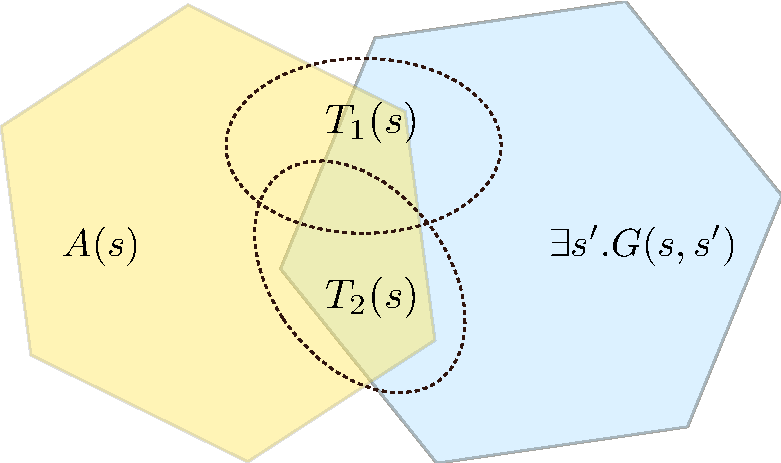
\includegraphics[width=2.5in]{aeval_invalid}
\caption{Region of validity computed for an example requiring \aeval to iterate two times.}
\label{fg:aeval}
\end{figure}

\aeval~\cite{fedyukovich2015automated} is an algorithm to decide validity and extract Skolem functions.
It takes as input a formula of the form $\forall s \,.\,  A(s) \Rightarrow \exists s' . G(s,s')$, 
where $A(s)$ has only existential\andreas{you meant universal here, right?} quantifiers, and $G(s,s')$ is quantifier-free.
%
While deciding the validity, \aeval iteratively enumerates models of $A(s) \land G (s, s')$ and groups them into a set of partitions $\{P_i(s)\}$, such that each $P_i(s) \Rightarrow \exists s' . G (s, s')$.
We say that after $n$ iterations, \aeval establishes a formula $R_n(s) \eqdef \bigvee_{i=1}^n P_i(s)$ which is by definition an under-approximation of $\exists s' . G (s, s')$.

If after $n$ iterations, it happens that $A(s) \Rightarrow R_n(s)$ then $\forall s \,.\,  A(s) \Rightarrow \exists s' . G(s,s')$ is valid, and \aeval generates a Skolem function as described in~\cite{katis2016synthesis}.
Alternatively, if $A(s) \land  G (s, s') \land \neg{R_n (s, s')}$ is unsatisfiable, then $A(s) \land \neg G (s, s')$ is satisfiable, or equivalently $\forall s \,.\,  A(s) \Rightarrow \exists s' . G(s,s')$ is invalid (see an example in Figure~\ref{fg:aeval}).
In both cases, we say that $A(s) \land R_n(s)$ is a \emph{region of validity}, meaning that $\forall s \,.\,  A(s) \land R_n(s) \Rightarrow \exists s' . G(s,s')$ is valid by construction.

\begin{lemma}
If formula $\forall s \,.\,  A(s) \Rightarrow \exists s' . G(s,s')$ is invalid, and $A(s) \land R_n(s)$ is the region of validity, then there is no other formula $S(s)$ such that $A(s) \land R_n(s) \Rightarrow S(s)$ and $\forall s \,.\,  S(s) \Rightarrow \exists s' . G(s,s')$.

\label{lem:subset}
\end{lemma}


\section{Validity-Guided Synthesis from Assume-Guarantee Contracts}
\label{sec:synthesis}

\begin{algorithm*}[!t]
\caption{\jsynvg (A : assumptions, G : guarantees)}
\label{alg:synthesis}
\begin{algorithmic}[1]
%\Procedure{\jsynvg}{A : assumptions, G : guarantees}
	\State $F(s) \gets true$;\Comment{Fixpoint of viable states}
	\While{true}
		\State $\phi \gets \forall s,i. \ (F(s) \land A(s,i) \Rightarrow \exists s'.G_{T}(s,i,s') \land F(s'))$;
		\State $\aevalres \gets \aeval(\phi)$;
%		\State $\tuple{\skolems, \subs} \gets \aeval(\phi)$;
		\If{$\isValid(\aevalres)$}
            \State{$\init \gets SAT(G_{I}(s) \land F(s))$}
            \If{$\isSat(\init) \ \land \ F(s) \neq  false$}
			%\If{$G_{I}(s) \land F(s) \neq false$}
		        \andreas{I'm not yet comfortable with the algorithm returning a model for the initial states. That could be misunderstood as the implementation starting from a single possible assignment. The Skolem may have multiple branches that may be used as initial state assignments\ldots}
				\Return $\tuple{\realizable, \aevalres.\skolems, init.model, F}$;
			\Else{\Comment{Empty set of initial or viable states}}
		 		\Return $\tuple{\unrealizable, \varnothing}$;
		 	\EndIf
		\Else{\Comment{Extract region of validity $Q(s,i)$}}
			\State $Q(s,i) \gets \aevalres.\subs$;
%			\If{$Q(s,i) = false$}
%				\Return $\tuple{\unrealizable, \varnothing}$;
%			\EndIf
			\State $\phi' \gets \forall s. \ (F(s) \Rightarrow \exists i. A(s,i) \land \lnot
			Q(s,i))$;
			\State $\aevalres' \gets \aeval(\phi')$;
%			\State $\tuple{\skolems', \subs'}\gets \aeval(\phi')$;
%			\If{$(\isValid(\phi'))$}\Comment{If $Q(s,i)$ contains only unsafe states}
%				\Return $\tuple{\unrealizable, \skolems'}$;
%			\Else{}\Comment{Extract witnessing cex}
			\State $W(s) \gets true$;
			\If{$\isInvalid(\aevalres')$}
				\State $W(s) \gets \aevalres.\subs'$;
			\EndIf
			\State $F(s) \gets F(s) \land \lnot W(s)$;\Comment{Refine set of viable states}	
			
%				\If{$W(s) = false$}
%					\Return $\tuple{\unrealizable, \varnothing}$;
%				\EndIf
				
%			\EndIf
		\EndIf
	\EndWhile
%\EndProcedure
\end{algorithmic}
\end{algorithm*}

The main contribution presented in this paper, is a novel idea that effectively
uses the information provided by regions of validity to compute a
greatest fixpoint of safe states. In our context, this fixpoint is not only
usable as a proof to the realizability of a specification, but also leads to the
construction of a witness that can be translated with a straightforward process
into a functional and efficient implementation. The algorithm is
presented in detail in Section~\ref{sec:alg} and we provide soundness
proofs regarding the algorithm's capabilities of determining the
realizability (unrealizability) of specification in
Section~\ref{sec:soundness}. An illustrative example is used in
Section~\ref{sec:example} to guide the reader through the process of
synthesizing implementations, using a specification that describes the Cinderella-Stepmother game.

\subsection{Algorithm}
\label{sec:alg}
Algorithm~\ref{alg:synthesis}, named \jsynvg, shows the validity-guided technique that we use towards the automatic synthesis of implementations. The specification is written using the Assume-Guarantee convention that we described in Section~\ref{sec:formals} and is provided as an input to the algorithm.
Line 1 initializes the process by defining the fixpoint $F(s)$ to be equal to
$true$. The algorithm then attempts to converge to a fixpoint $F(s)$
that only contains viable states, considering Equation~\ref{eq:viable}
and~\ref{eq:nonempty}.
We therefore construct the formula $\phi \gets \forall s,i. \ (F(s) \land A(s,i)
\Rightarrow \exists s'. G_{T}(s,i,s') \land F(s'))$, and provide it as an input to \aeval (Line 3). \aeval is particularly
focused on determining the validity of $\phi$. If the formula is valid, then a witness
\textit{Skolem} is constructed, containing valid assignments to the
existentially quantified variables of $\phi$. In the context of viability, this
witness is capable of providing viable states that can be used as a safe
reaction, given a prior viable state and an input that
satisfies the assumptions. With a valid formula at hand, it only remains to check that the fixpoint is not empty, and intersects with the initial states (Line 7).
If the check passes, we have a realizable contract and the algorithm returns the extracted witness that can be used as an implementation. Otherwise, the contract is unrealizable, since either the are no states that satisfy the
initial state guarantees $G_I$, or the set of viable states $F(s)$ is empty.

If $\phi$ is not true for every possible assignment of the universally
quantified variables, \aeval provides a \textit{region of validity} $Q(s,i)$
(Line 12).
%an exact subset of $F(s) \land A(s,i)$, namely $Q(s,i)$, which, if plugged in
% the original left-hand side of $\phi$, makes the resulting formula valid. We will refer to such subsets as \textit{regions of
%validity}.
At this point, one could falsely assume that replacing $F(s) \land A(s,i)$ with
$Q(s,i)$ is sufficient to solve our problem, and use the resulting witness as a
candidate implementation. This is not the case however, as $Q(s,i)$ is a subset
of both state and input variables. As such, it may contain further constraints
over the contract's inputs. This would lead to implementations that only
consider a subset of the original assumptions of the contract, with no
pre-defined strategy for the rest of the originally valid inputs.
Fortunately, we can exploit \aeval's capability of providing regions of validity
towards eliminating this issue.

The main concept to properly refine $F(s)$ is to extract a region of validity $W(s)$
that only involves constraints over state variables. To achieve this, we ask \aeval to determine
the validity of the formula $\phi' \gets \forall s. \ (F(s) \Rightarrow \exists
i. A(s,i) \land \lnot Q(s,i))$ (Line 13). If $\phi'$ is invalid, \aeval computes
a new region of validity and assigns it to $W(s)$. The new region is a strict subset of
$F(s)$, is described using constraints only over state variables, and entails
the existence of unsafe states in $F(s)$, considering valid inputs.
On the other hand, if $\phi'$ is a valid formula, then for any assignment of the state variables $s$, we have a valid input (i.e. that
satisfies the assumptions), for which the states are do not satisfy the constraints defined by the region
of validity $Q(s,i)$. This is a case of an unrealizable contract, as no state is
safe in this context and $W(s)$ gets assigned to $true$, eventually leading to a failed check in Line 7, during the next iteration.

Assuming that a region of validity is extracted ($W(s) \neq true$) we can finally refine $F(s)$, by conjucting to it the negation of $W(s)$ (Line 18).
Despite the fact that we now have a refined set of viable states, we are not yet done,
as $\lnot W(s)$ is not an exact region of validity, with respect to $Q(s,i)$. As
such there might still be states in $Q(s,i)$ that are not covered by $\lnot W(s)$. Therefore, we reiterate the
process by repeating the top-level \aeval query, with $F(s) \gets F(s) \land \lnot
W(s)$. Eventually, we either reach a greatest fixpoint $F(s)$ that effectively
describes the set of viable states, or reach the case where $F(s) = false$, and
declare our contract to be unrealizable.

\subsection{Notes}

\mike{Here are my notes...sorry that these are disorganized}
Things to fix:
\begin{itemize}
\item The initial state is not returned by the algorithm.
\item The algorithm checks for validity of $\phi$, but isn't this the same as checking whether the viable region is valid?  Does this boil down to checking whether viableRegion == true?
\item We need to know where to start a proof.  If it is in terms of the result of Algorithm 1, then it needs to be something returned by Algorithm 1.
\end{itemize}

%If the algorithm terminates with a $\realizable$ result, it is straightforward to establish that the generated Skolem function yields a realization.

Lemmas / proof thoughts.  For soundness of realizable results:
\begin{itemize}
    \item It is straightforward to show $Viable$ of the initial state proposed by
        the algorithm, just by the definition of the fixpoint function, but this doesn't really show the correctness of the Realization (Transition system).
    \item Showing Realization would be more interesting.
    \item $\reachable_{A}(s) \implies F(s)$.  We can prove this with induction.  Base case is easy. Showing inductive case: $\reachable_{A}(s') \implies F(s')$ from pre-state is also, I think straightforward from:
        \begin{itemize}
            \item $\reachable_{A}(s) => F(s)$
            \item $\reachable_{A}(s)$
            \item $A(s, i)$
            \item $T(s, i, s')$
        \end{itemize}
        so this immediately implies $F(s')$
    \item Now we can address the Realization claims, which are all simple non-inductive proofs that follow from definition that T satisfies our fixpoint formula.
\end{itemize}

For soundness of unrealizable results:
\begin{itemize}
    \item Show Algorithm 1 yields a greatest fixed point
    \item Show each iteration removes only states that are known to yield a violation.  This is where exactness of AEval is necessary.  This may be a delicate argument; I have not thought it through yet.  I think it would be proved via induction: something like, for each loop iteration, if $\lnot F$ contains only
        states that violate the guarantees under the assumptions, then $\lnot F'$ contains only states that violate the guarantees under the assumptions.
\end{itemize}

Put these two results together and we have that the algorithm yields correct results when it terminates (partial correctness).

Furthermore, for finite-state problems, the algorithm is totally correct.  For this, we need another proof leg:
\begin{itemize}
    \item Each iteration removes at least one state from $F$.  (Progress)
\end{itemize}

\mike{End of Mike's notes}

\subsection{Soundness of Realizable Results}


\begin{lemma} $\reachable_A(s) \implies F(s)$
\end{lemma}

\begin{theorem} If Algorithm~\ref{alg:synthesis} terminates with $\tuple{\realizable, \skolems, I, F}$, then it is a {\em Realization} of the contract $(A, (G_{I}, G_{T}))$.
\end{theorem}


\subsection{Soundness of Unrealizable Results}


\begin{lemma}
$\viable(s) \implies s \in F$ is a loop invariant for Algorithm~\ref{alg:synthesis} line (2).
\label{lem:alg1-viable}
\end{lemma}

\begin{corollary}
$s \notin F \implies \lnot \viable(s)$ is a loop invariant for Algorithm~\ref{alg:synthesis} line (2).
\label{cor:alg1-nonviable}
\end{corollary}

\begin{proof}
Immediate from Lemma~\ref{lem:alg1-viable}.
\end{proof}

\begin{theorem} If Algorithm~\ref{alg:synthesis} terminates with $\tuple{\unrealizable, ?}$, then there is no $Viable$ state $s$.
\end{theorem}

Perhaps we don't even need to bring in Tarski...It could be done with just Hoare logic loop invariants.

\subsection{Termination on Finite Models}

\begin{lemma}
Every loop iteration in Algorithm~\ref{alg:synthesis} either terminates or removes at least one state from $F$.
\end{lemma}

\begin{theorem}
For finite models, Algorithm~\ref{alg:synthesis} terminates.
\end{theorem}




\iffalse
The system $\mathfrak{U} = \tuple{S, \subseteq}$ is a complete lattice, where every subset $S' \subseteq S$ has a greatest lower bound  $\glb(S') = \cap S'$  and a least upper bound $\lub(S') = \cup S'$.
\label{lem:altlattice}
%\end{lemma}
\fi
\begin{proof}
Since the inclusion relation $\subseteq$ has been established over $S$, every subset $S' = \{M_k, M_{k+1}, \ldots M_{k+n}\}, n \in \mathbb{N}$ has a $\glb(S') = M_{k-1}$ and a $\lub(S') = M_{k+n+1}$. For the special case where $S' = S$ we have that $\glb(S) = M_0 = false$ and $\lub(S) = true$.
\end{proof}

\label{sec:soundness}
To prove Algorithm~\ref{alg:synthesis}'s soundness regarding results, we first need to show that the algorithm always computes a fixpoint containing only state variable assignments that lead to the satisfiability of $\forall\exists$-formulas following the form of Equation~\ref{eq:viable}. To achieve this, we
use Tarski's fixed point theorem~\cite{tarski1955lattice}.


%\andreas{An alternative would be to define a set S where each element is a set X of valid regions that lead to SAT, and the order in which X elements are constructed to be the relation that establishes a partial order over S. I have included these alternative theorems in an iffalse block in the .tex file. Please let me know which seems better tou you.}

We define the set $S = \{M_k, \ k \in \mathbb{N} \land \forall s, i. \ (M_k(s) \land A(s,i) \Rightarrow \exists s'. G_T(s,i,s') \land M_k(s'))\}$. In other words, $S$ is the set of subsets $M_k$, $k = 0, 1 , \ldots$ that contain constraints to states $s$, such that the formula $\forall s, i. \ (M_k(s) \land A(s,i) \Rightarrow \exists s'. G_T(s,i,s') \land M(s'))$ is satisfiable. The binary relation $\subseteq$ establishes a partial order on $S$, such that for any $k$, $M_k \subseteq M_{k+1}$.

\begin{lemma} The system $\mathfrak{U} = \tuple{S, \subseteq}$ is a complete lattice, where every subset $S' \subseteq S$ has a greatest lower bound  $\glb(S') = \cap S'$  and a least upper bound $\lub(S') = \cup S'$.
\label{lem:altlattice}
\end{lemma}
\begin{proof}
Since the inclusion relation $\subseteq$ has been established over $S$, every subset $S' = \{M_k, M_{k+1}, \ldots M_{k+n}\}, n \in \mathbb{N}$ has a $\glb(S') = M_{k-1}$ and a $\lub(S') = M_{k+n+1}$. For the special case where $S' = S$ we have that $\glb(S) = M_0 = false$ and $\lub(S) = true$.
\end{proof}

\begin{lemma} Algorithm~\ref{alg:synthesis} is a monotonic function on $S$ to $S$.
\label{lm:altmonotonicity}
\end{lemma}
\begin{proof}
Algorithm~\ref{alg:synthesis} recursively reduces the region $S = true$ attempting to reach a greatest fixpoint of viable states $F(s)$, such that the formula $\forall s, i. (F(s) \land A(s,i) \Rightarrow \exists s'. G_T(s,i,s') \land F(s')$ is valid. Notice the difference between $F(s)$ and subsets $M_k$, since the former implies a stronger property over the $\forall\exists$-formula (validity over satisfiability). Initially $F(s) = S = true$, and the algorithm proceeds to compute a new set of viable states. During each iteration, we use $F(s)$ to store this set, and it is the case that for any iteration $i$ of the algorithm, $F_{i+1}(s) \subseteq F_{i}(s)$. As such, we can consider Algorithm~\ref{alg:synthesis} as an isotone, and more specifically increasing function $f$ since for any pair of viable sets $F_{i}, F_{i+1}$, if $F_{i+1} \subseteq F_{i}$, we have that $f(F_{i+1} \subseteq f(F_{i}))$.
\end{proof}

\begin{theorem}[Characterization of Generated Fixpoints]
The set $P$ of all fixpoints in Algorithm~\ref{alg:synthesis} is non
empty, and the system $\tuple{P, \subseteq}$ is a complete lattice.
\label{thm:altfixpoint}
\end{theorem}
\begin{proof}
The proof relies on Tarski's first theorem on fixed
points~\cite{tarski1955lattice}.
Considering Lemmas~\ref{lem:altlattice} and~\ref{lem:altmonotonicity}, we satisfy the first two
conditions of Tarski's theorem. When the specification is realizable, a
fixpoint is reached by Algorithm~\ref{alg:synthesis}, since each consecutive
attempt to further refine $F(s)$ results in the same set. On the other hand, if
the specification is unrealizable, the algorithm returns the fixpoint $F(s) = false$. Therefore, the
set $P$ of all fixpoints in Algorithm~\ref{alg:synthesis} contains at least two
fixpoints. The top-down refinement of the region $S = true$ ensures that the generated fixpoint is always the greatest fixpoint.

Since all three conditions of Tarski's Fixed Point theorem are satisfied by our
solution, we can conclude that $P$ is a non empty set, while the system
$\tuple{P, T}$ is a complete lattice, as it contains a \lub, which is
the solution to a realizable contract, while $\glb = false$, and corresponds to
the solution for an unrealizable contract.
\end{proof}


\iffalse
\begin{lemma} Consider the system
$\mathfrak{U} = \tuple{S, T}$. With $S$, we denote the set of
subsets of the orignal state space, such that each subset contains assignments that lead to the
satisfiability of Equation~\ref{eq:viable}. $T$ refers to the
transition relation between any two states, that establishes a partial order
on $S$. Then $\mathfrak{U}$ is a complete lattice, where every subset $B \subseteq
S$ has a greatest lower bound  $\glb = \cap B$  and a least upper
bound $\lub = \cup B$.
\label{lem:lattice}
\end{lemma}
\begin{proof}
Considering the partial order that is established by T, it is straightforward
to show that all subsets $B$ of $S$ contain a \glb and a \lub. These
are respectively, the states which have no preceeding state in $B$ other than
possible ones in the \glb, and the states from which we take a transition into
a new state that's either in the \lub, or outside of $B$. For the special case
where $B = S$, we have that $\glb = false$ and $\lub = true$.
\end{proof}

\john{I really do not follow this proof. Why is it clear that $T$ represents a partial order of states? Is $T$ the result of the synthesis algorithm? Certainly you could have a transition system in which states transition from one back to another and so on and so forth.}


\begin{lemma} Algorithm~\ref{alg:synthesis} is a monotonic function on $S$ to
$S$.

\john{The type of Algorithm~\ref{alg:synthesis}'s input is different from its output so I do not understand how it can map $S$ to $S$}.
\label{lem:monotonicity}
\end{lemma}
\begin{proof}
The algorithm recursively reduces $S$, attempting to reach a fixed point
at which $S$ only contains state assignments that lead to the satisfiability of
Equation~\ref{eq:viable}. As such, it can be considered as an isotone function
$f$, where, for every pair $(B,A)$ with $B \subseteq A \subseteq S$, we have that
$f(B) \subseteq f(A)$.
\end{proof}

\begin{theorem}[Characterization of Generated Fixpoints]
The set $P$ of all fixpoints in Algorithm~\ref{alg:synthesis} is non
empty, and the system $\tuple{P, T}$ is a complete lattice.
\label{thm:fixpoint}
\end{theorem}
\begin{proof}
The proof relies on Tarski's first theorem on fixed
points~\cite{tarski1955lattice}.
Considering Lemmas~\ref{lem:lattice} and~\ref{lem:monotonicity}, we satisfy the first two
conditions of Tarski's theorem. When the specification is realizable, a
fixpoint is reached by Algorithm~\ref{alg:synthesis}, since each consecutive
attempt to further refine $F(s)$ results in the same set. On the other hand, if
the specification is unrealizable, the algorithm returns the fixpoint $F(s) = false$. Therefore, the
set $P$ of all fixpoints in Algorithm~\ref{alg:synthesis} contains at least two
fixpoints.

Since all three conditions of Tarski's Fixed Point theorem are satisfied by our
solution, we can conclude that $P$ is a non empty set, while the system
$\tuple{P, T}$ is a complete lattice, as it contains a \lub, which is
the solution to a realizable contract, while $\glb = false$, and corresponds to
the solution for an unrealizable contract.
\end{proof}
\fi

From Theorem~\ref{thm:fixpoint} we have shown that Algorithm~\ref{alg:synthesis} computes a fixpoint for both cases where the specification is realizable or not. With this knowledge at hand, it is necessary to prove the soundness of the fixpoints generated. In other words, when a fixpoint is computed for a realizable contract, it should be the case that the algorithm reports a ``realizable'' result. The same needs to hold for the dual case of ``unrealizable'' results.

\begin{theorem}[Soundness of ``realizable'' results]
\label{thm:sndreal}

Assume a sound quantifier elimination process that provides us with exact regions of validity. If $F(s)$ is a fixpoint generated by Algorithm~\ref{alg:synthesis} and $F(s) \neq false$, then the contract is realizable.
\end{theorem}
\begin{proof} To prove this theorem, we show that $\forall s. \viable(s) \Rightarrow F(s)$ using induction on $F(s)$. The base case is covered since $F(s) \land G_I(s) \neq \varnothing$. For the inductive case, we require that a state $x$ exists, such that $G_T(s,i,x) \land F(x)$. Since $\viable(s)$ is true, we know that $\exists s'. G_T(s,i,s') \land \viable(s')$. Thus we pick $s'$ and use the inductive hypothesis to show that $\viable(s') \Rightarrow F(s')$.
\end{proof}

\john{The base case of this proof does not imply that $\exists s. \viable(s) \Rightarrow F(s)$. Viability is not defined in terms of $G_I(s)$. Also, even if you can show the base case is satisfied you need to make an assumption that $A(s,i)$ is non-empty in order to have $\exists s'. G_T(s,i,s') \land \viable(s')$. Also to imply induction this way don't we need to show that $\forall_i. G_T(s,i,s')$ is some sort of well-founded relation over $S$?}

\begin{theorem}[Soundness of ``unrealizable" results]
\label{thm:sndunreal}

Assume a quantifier elimination process that provides exact regions of validity. If the output of Algorithm~\ref{alg:synthesis} is the fixpoint $F(s) = false$, then the contract is unrealizable.
\end{theorem}
\begin{proof}
Dually to Theorem~\ref{thm:sndreal} we show that $\forall s. \lnot \viable(s) \Rightarrow \lnot F(s)$ using induction on $F(s)$. From this point on, the proof direction is analogous to that of Theorem~\ref{thm:sndreal}.
\end{proof}


\begin{corollary}[Soundness of Realizability results from Validity-Guided Synthesis]
Assume a quantifier elimination process that provides exact regions of validity. The process described in Algorithm~\ref{alg:synthesis} is sound.
\end{corollary}

Notice how the Theorems on the soundness of the results provided by the validity-guided approach assume a quantifier elimination process that computes exact regions of validity. This is a crucial requirement, as it determines the overall effectiveness of the approach. The algorithm is still applicable to cases where the assumption is not met, however its effectiveness on providing sound results is directly affected. Not considering the case of exact regions, we have two other cases, overapproximations and underapproximations. In the former case, the regions of unsafe states (i.e. the negation of a region of validity) would be underapproximations and the algorithm's performance decreases, since problems might not be solvable as fast as with the use of exact regions. On the other hand, if the regions of validity are underapproximations, their negations are overapproximations, and as such, the blocked regions might cover safe states in their constraints. This makes the algorithm follow a more pessimistic approach, where it overconstrains the problem to find a solution. This might lead to cases where an otherwise realizable contract might be declared as unrealizable by the process. We show how the latter can be manifested in practice in Section~\ref{sec:results}, where we compare our approach to a synthesis algorithm that is based on k-induction and is prone to incorrect ``unrealizable'' results. In the context of this paper, and considering Lemma~\ref{lem:subset}, \aeval is able to provide exact regions of validity.

\subsection{Applying \jsynvg to the Cinderella-Stepmother game}
\label{sec:algexample}

\begin{figure}[!t]
\centering
 \begin{Verbatim}[fontsize=\footnotesize]
const C = 2.0;

-- empty buckets e and e+1 each round
node game(i1,i2,i3,i4,i5: real; e: int)
	returns (guarantee: bool);
var
  b1, b2, b3, b4, b5 : real;
let
  assert i1 >= 0.0 and i2 >= 0.0 and
 	i3 >= 0.0 and i4 >= 0.0 and i5 >= 0.0;
  assert i1 + i2 + i3 + i4 + i5 = 1.0;

  b1 = 0.0 ->
       (if (e = 5 or e = 1) then i1
                            else (pre(b1) + i1));
  b2 = 0.0 ->
       (if (e = 1 or e = 2) then i2
                            else (pre(b2) + i2));
  b3 = 0.0 ->
       (if (e = 2 or e = 3) then i3
                            else (pre(b3) + i3));
  b4 = 0.0 ->
       (if (e = 3 or e = 4) then i4
                            else (pre(b4) + i4));
  b5 = 0.0 ->
       (if (e = 4 or e = 5) then i5
                            else (pre(b5) + i5));

  guarantee = b1 <= C and b2 <= C and b3 <= C and
  	    b4 <= C and b5 <= C;

  --%REALIZABLE i1, i2, i3, i4, i5;
  --%PROPERTY guarantee;
tel;
 \end{Verbatim}
\caption{An Assume-Guarantee contract for the Cinderella-Stepmother game in Lustre}
\label{fg:cind}
\end{figure}

Figure~\ref{fg:cind} shows one possible interpretation of the contract designed
for the instance of the Cinderella-Stepmother game that we introduced in Section~\ref{sec:example}. The contract
is expressed using Lustre~\cite{lustrev6}, a language
that has been extensively used for specification as well as implementation of
safety-critical systems, and is the kernel language in SCADE, a popular tool in
model-based development. The contract is defined as a Lustre node, with a global
constant $C$ denoting the bucket capacity. The node describes the game itself,
through the problem's input and output variables. The main input is Stepmother's
distribution of one unit of water over five different input variables,
\textit{i1} to \textit{i5}. While the node contains a sixth input argument,
namely $e$, this is in fact used as the output of the system that we want to
implement, representing Cinderella's choice at each of her turns. We make an
explicit distinction on which node arguments are the system's inputs, using the \textit{REALIZABLE} statement towards the end of the contract. The contract's
assumptions $A$ are defined using assertions over the input variables
\textit{i1-i5}. We assume that there can be no negative input values, and the
sum of \textit{i1} to \textit{i5} is equal to one unit of water. The specified node
returns the value of a boolean variable \textit{guarantee}, which corresponds to
the contract's guarantee $G$, and is explicitly defined to be such using the
\textit{PROPERTY} statement.
Finally, we define what each bucket's state should be through the entire
duration of the game, using the local variables \textit{b1} to \textit{b5}.
Initially, each bucket is empty, and with each transition to a new state, the contents depend on
whether Cinderella chose the specific bucket, or an adjacent one. If this is the
case, the contents of the bucket $b_i$ become equal to the amount of water that
Stepmother puts in the corresponding input variable $i$, during the next turn.
If the bucket was not covered by Cinderella's choice, then its contents are
updated by adding Stepmother's distribution to the volume of water that the
bucket already had. The distinction between the initial state of each bucket,
and every other state is expressed using Lustre's arrow (\texttt{->})
operator, while variable values in previous states can be accessed using the
\textit{pre} operation.
The specification is fairly simple, as the objective is clear. The contract
should only be realizable if, assuming valid inputs given by the Stepmother
(i.e. positive values to input variables that add up to one water unit),
Cinderella can keep reacting indefinitely, by providing outputs that satisfy the
guarantees (i.e. she empties buckets in order to prevent overflow in Stepmother's next turn).
We initiate our call to the procedure defined in Algorithm~\ref{alg:synthesis},
by providing the contract in Figure~\ref{fg:cind} as input. The algorithm
then enters an infinite loop, where it attempts to construct a fixpoint of
viable states that can use the transition relation to new, viable states,
while complying to the specification. Initially $F(s) = true$, and we ask \aeval for the validiity of the formula $\phi \gets \forall s,i. \ (F(s) \land A(s,i) \Rightarrow \exists s'.G_{T}(s,i,s') \land F(s'))$. Unfortunately, not every state in $F(s)$
satisfies the formula. As such $\phi$ is not valid, and \aeval provides us with
a region of validity $Q(s,i)$, which is a subset of $F(s) \land A(s,i)$ for
which the formula $\phi$ is valid. Since $Q(s,i)$ is defined over both state and
input variables, it might contain contraints over the inputs, which is an
undesirable side-effect. Due to space restrictions, we are unable to show this
in full effect, but Figure~\ref{fg:snippet} shows part of the generated
$Q(s,i)$, in SMT-LIB format (pre-fix notation), where the input variables are
part of the constraints. The variable \textit{\%init} is used in the underlying
machinery as a flag to indicate whether the current state is initial or not
(true and false, respectively). \andrew{Is there anything else we can
  say about the code in the figure? Does it give us any insight into a
  possible solution for cinderella?}

\begin{figure}[!t]
\centering
 \begin{Verbatim}[fontsize=\footnotesize]
(and (or (and %init (= (+ b1 i1) 0.0)) (not %init))
  (or (and %init (= (+ b2 i2) 0.0)) (not %init))
  (or (and %init (= (+ b3 i3) 0.0)) (not %init))
  (or (and %init (= i4 0.0)) (not %init))
  (or (and %init (= i5 0.0)) (not %init))
  (<= (+ b1 i1) 2.0)
  (<= (+ b2 i2) 2.0)
  (<= (+ b3 i3) 2.0)
  (<= i4 2.0)
  (<= i5 2.0))
 \end{Verbatim}
\caption{Code snippet of the region of validity generated for the Cinderella-Stepmother
example}
\label{fg:snippet}
\end{figure}

Considering the existence of undesirable constraints in $Q(s,i)$, the next step
is to extract a region of validity that is only described using state variables.
As such, we construct the formula $\phi' \gets \forall s. \ (F(s) \Rightarrow \exists
i. A(s,i) \land \lnot Q(s,i))$, and ask \aeval regarding its validity. According
to \aeval, $\phi'$ is not valid, an indication that may eventually lead us to a
proof of the contract's realizability. If $\phi'$ was valid, then every state in
$F(s)$ is unsafe, under a specific input that satisfies the contract
assumptions (since $\lnot Q(s,i)$ holds in this case), and the specification is unrealizable. Since this is not the case,
however, \aeval computes a region of validity $W(s)$ that describes states that are unsafe under certain valid inputs. As a consequence, a refinement process comes at the next step. in which we derive $F(s) = F(s) \land \lnot W(s)$, thus blocking the unsafe region $W(s)$.

From this point on, the algorithm reiterates the process following the steps
explained above. For this particular example, the algorithm terminates after one
more refinement, at depth 2. At that point, the refined version of
$\phi$ is valid, and \aeval constructs a witness containing valid reactions to
environment behavior. Figure~\ref{fg:witness} provides a snippet of
that witness, after being translated to a C implementation. \andrew{What's with the 'if' in the middle of the 'else' block? Is it
  suppose to be an 'else-if'?}
In general,
the witness is described through the use of an nested if-then-else block, where the conditions are subsets of the antecedent of
the implication in formula $\phi$, while the body contains valid assignments to
state variables, for this particular subset.


\begin{figure}[!t]
\centering
 \begin{Verbatim}[fontsize=\footnotesize]
...
if (!(b1 + i1 <= 0.0) || !((b2 + i2) <= 0.0) || ...)
  e = 3;
  b1 = b1 + i1;
  b2 = b2 + i2;
  b3 = i3;
  b4 = i4;
  b5 = b5 + i5;
} else {
  if (!(i1 <= 0.0) || !((b2 + i2) <= 0.0) || ...)
  e = 5;
  b1 = i1;
  b2 = b2 + i2;
  b3 = b3 + i3;
  b4 = b4 + i4;
  b5 = i5;
} else {
...
 \end{Verbatim}
\caption{Code snippet of the synthesized implementation for the Cinderella-Stepmother
example}
\label{fg:witness}
\end{figure}

As is discussed by Beyene \textit{et al.}~\cite{beyene2014constraint}, the
Cinderella-Stepmother is a rather challenging game. In particular, for the
cases where $1.5 \leq C \leq 3.0$, the problem becomes non-trivial, and their
work showed how familiarity with the problem can help alleviate this complexity
through the use of pre-defined templates. Despite this, we were still
able to synthesize implementations for the Cinderella-Stepmother game for any
value of $C \geq 2$, using a completely automatic approach.~\footnote{The region $1.5\leq C < 2$ is a particularly hard problem and the algorithm does not converge with a timeout up to seven hours.} This fact alone,
provided us with solid foundations regarding the algorithm's effectiveness in
solving complex problems.

\section{Implementation and Evaluation}
\label{sec:impl}

The implementation of the algorithm has been added to a branch of the  \jkind~\cite{jkind} model checker.  \jkind officially supports synthesis
%\grigory{Unofficially? We have the Tech Report, it is all official ;)}
using a k-inductive approach, named \jsyn~\cite{KatisFGBGW16}. For clarity, we named
our validity-guided technique \jsynvg. \jkind uses Lustre~\cite{lustrev6} as its specification and implementation language.
\iffalse
, which functions as an intermediate representation to the Architecture Analysis and Design Language (\textsc{AADL})~\cite{feiler2006architecture}.
The latter is a high-level specification and analysis language with which
contracts are expressed, using the Assume-Guarantee Reasoning (\textsc{AGREE})
framework~\cite{NFM2012:CoGaMiWhLaLu}.
\andrew{it seems strange to be talking about AADL and maybe even AGREE  at all here.}

\fi
%
%\footnote{An unofficial release of \jkind
%including our synthesis algorithm is available to download at
%https://github.com/andrewkatis/jkind-1/tree/synthesis. \aeval needs to be
%installed separately from https://github.com/grigoryfedyukovich/aeval.}.
%During the internal process, 
\jsynvg encodes Lustre specifications in the language of
linear real and integer arithmetic (LIRA)
% first order logic 
and communicates them to \aeval.
%f the SMT-LIB language,
%, with which the $\forall\exists$-formulas, regions of
%validity, as well as the witnesses are expressed.
%The underlying solver that is
%used is the \aeval Skolemizer, 
%which currently supports
%$\forall\exists$-formulas expressed using 
%linear real and integer arithmetic (LIRA).
%
%
%For realizable specifications, and considering Alg.~\ref{alg:synthesis}, we
%recursively use regions of validity to block out unsafe states from the search
%space.
%Eventually, we reach a fixpoint that is sufficient to use in order to extract a 
Skolem functions returned by \aeval get then translated %that witnesses the realizability of the specification. Given
%the generated function, what remains is its translation
into an efficient and practical implementation. To compare the quality of implementations against \jsyn, we use
\smtlibtoc, a tool that has been specifically developed to translate
  Skolem functions to C implementations.
%\grigory{There used to be a rehash of Alg.~\ref{alg:synthesis}; no need to repeat it here.}
%\grigory{Also, you probably need to refer the reader that more info about implementation is in~\cite{KatisFGBGW16}.}

%In future work,
%we intend to further improve on this, and
%many other aspects of the compiler's performance as part of an individual
%future work.



%%% Local Variables:
%%% mode: latex
%%% TeX-master: "document"
%%% End:

\section{Experimental Results}
\label{sec:results}

\begin{figure}[!t]
\centering
\subfloat[Performance Comparison]{
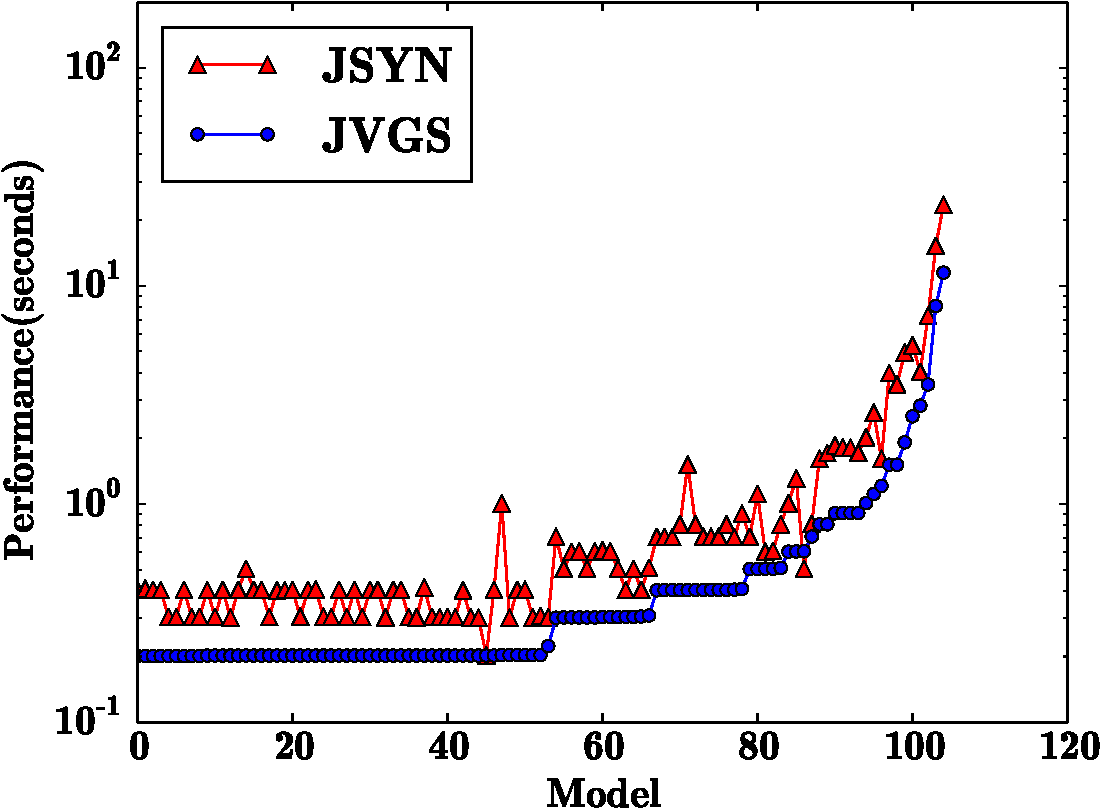
\includegraphics[width=3in]{overhead-crop}
\label{fg:performance}}
%\hspace{+6.5em}

\subfloat[Size of Synthesized
Implementations]{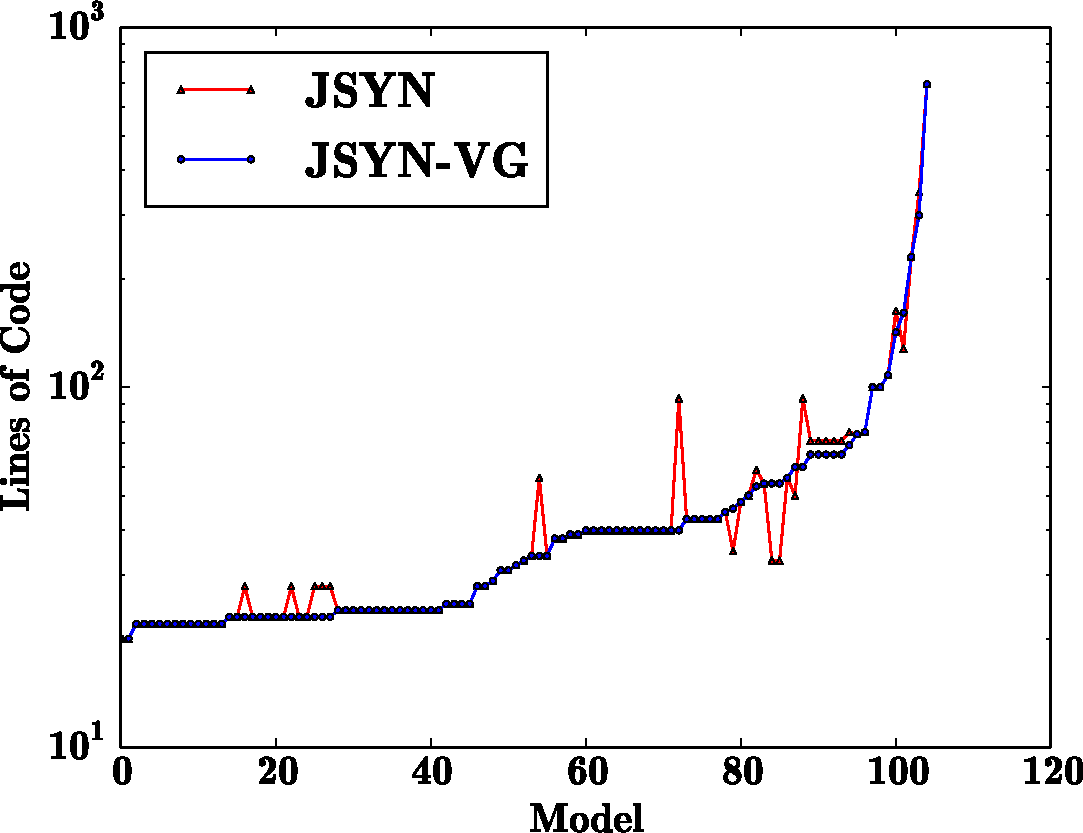
\includegraphics[width=3in]{loc-crop}
\label{fg:size}}

\subfloat[Performance of Synthesized Implementations]{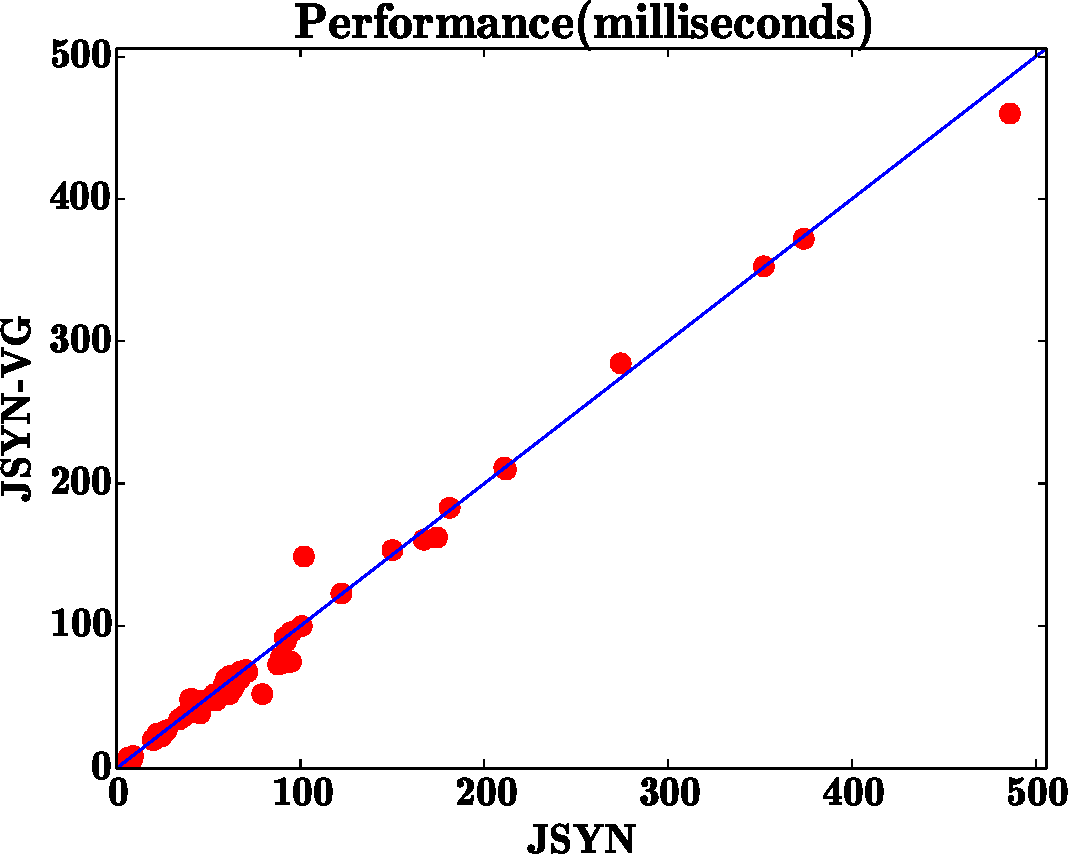
\includegraphics[width=3in]{performance-crop}
\label{fg:implperformance}}
\caption{Experimental results}
\label{fg:results}
\end{figure}

In this section we evaluate \jsynvg by synthesizing implementations
for 110 contracts that originate from a broad variety of contexts.~\footnote{An
anonymized repository containing the benchmark contracts can be found at
\url{https://tinyurl.com/mjtyxae }. We will replace this repository with the official for the camera-ready
version of the paper.} Almost half of them, 54, come from a collection of contracts that were initally used for the verification of existing handwritten implementations. The second biggest collection in our suite contains 52 contracts that correspond to various development projects, such as a Quad-Redundant Flight Control System, a Generic Patient Controlled Analgesia infusion pump, as well as a collection of contracts
for a Microwave model, written by graduate students as part of a software
engineering class. The remaining nine models contain variations of the
Cinderella-Stepmother game and the example in Section~\ref{sec:pre}.

Since \jkind already supports synthesis through \jsyn, we were able to directly
compare \jsynvg against \jsyn's k-inductive approach.
The comparison spans over multiple factors, including
algorithm performance, number of problems solved and, finally, performance
of C implementations through the translation of witnesses using \smtlibtoc. We
ran the experiments using a computer with Intel Core i3-4010U 1.70GHz CPU and
16GB RAM.

\begin{table}[!t]
\centering
\caption{Benchmark Statistics}
\label{tbl:stats}
\begin{tabular}{@{}lll@{}}
\toprule
 & \jsyn & \jsynvg \\ \midrule
Problems solved & 110 & \textbf{115} \\
Performance (avg - seconds) & 2.71 & \textbf{1.24} \\
Performance (max - seconds) & 159.05 & \textbf{64.89} \\
Implementation Size (avg - Lines of Code) & 74.45 & \textbf{69.77} \\
Implementation Size (max - Lines of Code) & 2382 & \textbf{2062} \\
Implementation Performance (avg - ms) & \textbf{56.57} & 58.47 \\
Implementation Performance (max - ms) & \textbf{464.359} & 485.197 \\
\bottomrule
\end{tabular}
\end{table}


\begin{table*}[!t]
\centering
\caption{Cinderella-Stepmother results}
\label{tbl:cindtbl}
\begin{tabular}{|c|c|c|c|c|c|}
\hline
 & \multicolumn{3}{c|}{JSYN-VG} & \multicolumn{2}{c|}{CONSYNTH~\cite{beyene2014constraint}} \\ \hline
 & Implementation Size (LoC) & Implementation Performance (ms) & Time & Time (Z3) & Time (Barcelogic) \\ \hline
Cinderella (C = 3) & 92 & 262.84 & 35s & \multirow{3.2s} & \multirow{1.2s} \\ \cline{1-4}
Cinderella2 (C = 3) & 222 & 309.24 & 2m9s &  &  \\ \hline
Cinderella (C = 2) & 102 & 196.57 & 24s & \multirow{1m52s} & \multirow{1m52s} \\ \cline{1-4}
Cinderella2 (C = 2) & 272 & 230.16 & 2m9s &  &  \\ \hline
\end{tabular}
\end{table*}

A listing of the statistics that we tracked while running experiments is
presented in Table~\ref{tbl:stats}.
Figure~\ref{fg:performance} shows the time allocated by \jsyn and \jsynvg to solve each problem, with \jsynvg
outperforming \jsyn across the board, often times by a margin greater than
50\%. Figure~\ref{fg:size} on the other hand, depicts small differences in the
overall size between the synthesized implementations. While it would be
reasonable to conclude that there are no noticable improvements, the bigger
picture is different. The key factor that is not apparent from this figure, is the length of the k-inductive proof. For the majority of the benchmarks in the suite, \jsyn proves their realizability by constructing proofs of length $k=0$, which essentially means
that the entire space of states is an inductive invariant. As such, \jsynvg
also manages to synthesize implementations without requiring any refinement
process. For these cases, both algorithms generate a single Skolem function. In the general case though, the size of \jsyn solutions is directly
dependent on $k$, since each implementation is composed of $k$ Skolem
functions ($k-1$ to initialize the system, and one last for the inductive step),
where the equivalent solution from \jsynvg is always just one.
Figure~\ref{fg:size} hints towards this intuition, through a handful of spikes
in \jsyn implementation size. Despite this, we also noticed cases where \jsyn
implementations are shorter. This provides us with another interesting
observation regarding the formulation of the problem for $k=0$ proofs. In
these cases, \jsyn proves the existence of viable states, starting from a set
of \textit{pre-initial} states, where the contract does not need to hold. This
has direct implications to the way that the $\forall\exists$-formulas are
constructed in \jsyn's underlying machinery, where the assumptions are ``baked''
into the transition relation, affecting thus the creation of Model-Based
Projections by \aeval.

 One last statistic that we tracked was the performance of the synthesized C
 implementations, which can be seen in Figure~\ref{fg:implperformance}. For this purpose, we translated the
 generated witnesses from \jsyn and \jsynvg solutions using
 \smtlibtoc under the same set of options. Table~\ref{tbl:stats} shows that
 while \jsyn implementations are faster, the difference is minuscule on average. 
This may be in part because \jsyn creates separate skolem functions for the initial evaluation (when \%init is true) and subsequent evaluations, whereas currently \jsynvg uses a single function for both the initial and subsequent steps.  We are considering specialization of the generated \jsynvg functions based on \%init, as well as several other optimizations of the generated code in future work.

 
% The deciding factor in this context is the
% difference in complexity of the Model-Based Projections that get generated by
% \aeval using \jsyn and \jsynvg, with the latter versions containing richer
% expressions, mainly due to the refinement process.

Figure~\ref{fg:results} does not cover the entirety of the
benchmark suite. From the original 110 problems, five of them cannot be
solved by \jsyn's k-inductive approach. Four of these files are variations of
the cinderella-stepmother game that we described in Section~\ref{sec:example}, using different representations of the game, as well as two different values
for the bucket capacity (2 and 3). Using the variation that we included in the
aforementioned section as an input to \jsyn, we receive an ``unrealizable'' answer, with the counterexample shown
in Figure~\ref{fg:cex}. Reading through the feedback provided by \jsyn, it is
apparent that the underlying SMT solver is incapable of choosing the correct
buckets to empty, leading eventually to a state where an overflow occurs for the
third bucket. As we already discussed though, a winning strategy exists for the
cinderella, as long as the bucket capacity $c$ is between 1.5 and 3. This
provides an excellent demonstration regarding the inherent weakness of \jsyn
in providing sound ``unrealizable'' results. \jsynvg's validity-guided approach,
on the other hand, was able to prove the realizability for these contracts, as
well as synthesize an implementation for each.

\begin{figure}[!t]
\centering
 \begin{Verbatim}[fontsize=\scriptsize]
 ++++++++++++++++++++++++++++++++++++++++++++++++++++++++++
      UNREALIZABLE || K = 6 || Time = 2.017s
                 Step
      variable      0    1      2      3      4      5
      INPUTS
      i1            0    0      0 0.416* 0.944* 0.666*
      i2            1    0 0.083* 0.083*      0 0.055*
      i3            0    1 0.305*    0.5 0.027* 0.194*
      i4            0    0 0.611*      0      0 0.027*
      i5            0    0      0      0 0.027* 0.055*

      OUTPUTS
      e             1    3      1      5      4      5

      NODE OUTPUTS
      guarantee   true true   true   true   true  false

      NODE LOCALS
      b1            0    0      0 0.416* 1.361* 0.666*
      b2            0    0 0.083* 0.166* 0.166* 0.222*
      b3            0    1 1.305* 1.805* 1.833* 2.027*
      b4            0    0 0.611* 0.611*      0 0.027*
      b5            0    0      0      0 0.027* 0.055*

      * display value has been truncated
 +++++++++++++++++++++++++++++++++++++++++++++++++++++++++
 \end{Verbatim}
\caption{Spurious counterexample for Cinderella-Stepmother example using \jsyn}

\label{fg:cex}
\end{figure}

Table~\ref{tbl:cindtbl} shows how \jsynvg performed against the four contracts describing the Cinderella-Stepmother game. We used two different interpretations for the game, and exercised both for the cases where the bucket capacity $C$ is equal to 2 and 3. The performance is heavily affected when we exercise the variation for $C=2$, but \jsynvg is still able to synthesize a winning region for Cinderella. Regarding the synthesized implementations, their size remains analogous to the difficulty of the problem, in conjunction with the complexity of the program (Cinderella2 contains more local variables and a helper function to empty buckets). Despite this, the implementation performance remains at the same level across all the implementations. Finally for reference, the table contains the results from the template-based approach followed in \textsc{Consynth}~\cite{beyene2014constraint}. From the results, it is apparent that providing templates drammatically increases the performance of the underlying synthesis procedure. Nevertheless, the automated approach in \jsynvg is able to synthesize solutions for the same problems in a reasonable time margin, when compared to \textsc{Consynth}.


Overall, \jsynvg's validity-guided approach provides significant advantages
over the k-inductive technique followed in \jsyn, and effectively expands
\jkind's solving capabilities regarding specification realizability. On top of that, it provides an efficient ``hands-off'' approach that is capable of solving complex games.
The most significant contribution, however, is the applicability of this approach, as it is not tied to a specific environment since it can be extended to support more
theories, as well as categories of specification.

\section{Related Work}
\label{sec:related}

\iffalse
The alternative name to program synthesis is Church's problem, since the description of the problem was first described by Church in 1963~\cite{church1962logic}. Research in this field of program synthesis attributes began in the 1970s, when Manna and Waldinger~\cite{manna1971toward} first introduced a synthesis procedure using principles of theorem proving. Almost two decades later, Pnueliand Rosner~\cite{pnueli1989synthesis} first formally described the
implementability of reactive systems, considering first order logic formulas
that stem from temporal specifications. In the same work, they provided a
complete approach to synthesize finite-state implementations through the
construction of deterministic Rabin automata.

In the recent years, program synthesis has enjoyed a vast variety of
contributions under numerous contexts. Gulwani~\cite{gulwani2010dimensions}
presented an extended survey, hinting future research directions. Synthesis
algorithms have been proposed for simple LTL specification~\cite{Bohy12,Tini03}
subsets of it~\cite{Klein10,ehlers2010symbolic,cheng2016structural}, as well as under other temporal logics~\cite{monmege2016real,Hamza10}, such as SIS~\cite{Aziz95}.
Chatterjee and Henzinger~\cite{Chatterjee07} proposed a novel component-based approach using the notion of Assume-Guarantee contracts.
\fi
The work presented in this paper is closely related to approaches that attempt
to construct infinite-state implementations. Some focus on the continuous
interaction of the user with the underlying machinery, either through the use of
templates~\cite{srivastava2013template,beyene2014constraint}, or environments where the user attempts to guide the solver by choosing reactions from a collection of different
interpretations~\cite{ryzhyk2016developing}. We differentiate from this
direction by providing a completely automatic approach that does not require
human ingenuity to find a solution and most importantly, the user
does not need to be deeply familiar with the problem at hand.
\iffalse
 A ``hands-off'' approach has been proposed in the past by Katis \textit{et
al.}~\cite{gacek2015towards,katis2016towards,katis2016synthesis}. The work is
based on the concept of extracting collections of reactions that witness the satisfaction of a k-inductive proof on the contract's realizability.
In Section~\ref{sec:results} we were able to effectively show in practice how a
validity-guided approach significantly improves upon this work, by using a
fixpoint-generating technique rather than the principle of k-induction.
\fi

The technique in this paper follows similar directions on abductive inference~\cite{dillig2013inductive, dillig2014optimal}. Dillig \textit{et al.} showed how abduction can be used to build an inductive frame for invariant generation and guard synthesis. Their approach focuses on checking the validity of quantifier-free formulas of the form $\phi \implies \psi$ via a refinement process that generates candidate invariants in the form of maximum universal subsets (MUS).  While a MUS may be sufficient to prove validity, it may also mislead the invariant search, so the authors use a backtracking procedure that discovers new subsets while avoiding spurious results. By comparison, in our approach the regions of validity are maximal and therefore backtracking is not required.  More importantly, reactive synthesis requires mixed-quantifier formulas, and it requires that inputs are unconstrained (other than by the contract assumptions), so substantial modifications to the MUS algorithm would be necessary to apply the approach of~\cite{dillig2014optimal} for reactive synthesis.  %In our work, the ability to generate precise regions of validity lead to a very simple refinement process that is solely based on the input variables being existentially quantified.

The concept of synthesizing implementations by discovering fixpoints was mostly
inspired by the IC3 algorithm, the technique also known as Property Directed
Reachability~\cite{bradley2011sat,een2011efficient}, which was first introduced
in the context of verification. Work from Cimatti \textit{et al.} effectively
applied this idea for synthesis, albeit that of parameters, in the
\textsc{HyComp} model checker~\cite{DBLP:conf/fmcad/CimattiGMT13, cimatti2015hycomp}.
Discovering fixpoints to synthesize reactive designs was first
extensively covered by Piterman \textit{et al.}~\cite{piterman2006synthesis}
who proved that the problem can be solved in cubic time for the class of GR(1) specifications.
However, their proposed algorithm is significantly different from this paper. It
requires the discovery of least fixpoints for the state variables,
each one covering a greatest fixpoint of the input variables. If the specification
is realizable, then the entirety of the input space is covered by the greatest fixpoints. By comparison, we compute a single greatest fixpoint over the system's outputs, and we avoid the partitioning of the input space.  As the tools use different notations and support different logical fragments, comparisons are not straightforward; nevertheless we hope to perform a comparison in future work.

More recently, Preiner \textit{et al}. presented their work on counterexample-guided model synthesis (CEGMS)~\cite{preiner2017counterexample}. In CEGMS, candidate witnesses are being constructed and their validity is checked with respect to the specification. Internally, a counterexample-guided refinement process is used~\cite{reynolds2015counterexample} for the purposes of quantifier
elimination, and enumerative learning is applied to generalize witnesses. Enumerative learning is a syntax-based technique that enumerates expressions, checks their truth against
ground test cases, and proceeds to generalize the expressions by constructing larger ones. In constrast to the principle of enumerative learning, our approach is syntax-insensitive in terms of generating regions of validity.
\iffalse
On top of that, CEGMS has only been tested against the theory of Boolean Vectors (BV, and BV$_{LNIRA}$), while \jsynvg supports the mixed theories of linear integer and real arithmetic.
\fi
In general, enumeration techniques such as the one used in \textsc{ConSynth}'s underlying E-HSF engine~\cite{beyene2014constraint} is not an optimal strategy for our class of problems, since the witnesses constructed for the most complex contracts are described by nested if-then-else expressions of depth (i.e. number of branches) 10-20, a point at which space explosion is difficult to handle since the number of candidate solutions is significantly large.

\section{Conclusion and Future Work}
\label{sec:conclusion}

In this paper, we presented a novel and elegant approach towards the synthesis
of reactive system implementations, using only the knowledge provided by the
system specification expressed in linear integer and real arithmetic. The approach is
directly inspired from previous work on Property Directed Reachability, with the objective being the construction of inductive
invariants that can be used as a proof to the specification's realizability. The
main goal is to converge to a fixpoint by iteratively blocking subsets of
unsafe states from the problem space. This is achieved through the continuous
extraction of regions of validity which hint towards subsets of states that
lead to a candidate implementation.

This is the first complete attempt, to the best of our knowledge, on handling
valid subsets of a $\forall\exists$-formula to construct a greatest fixpoint,
while the specification is expressed using infinite theories. We were able to
prove its effectiveness in practice, by comparing it to an already existing
approach that focuses on constructing k-inductive proofs of realizability. The
results showed a dramatic improvement on performance, and indicated how the
validity-guided approach can lead to the solution of a bigger class of problems.

Future work in this area is rich with challenges and promising directions. The
most interesting question is how we can possibly improve \jsynvg's
speed of convergence. Not excluding techniques such as counterexample-guided
refinement and predicate abstraction~\cite{walker2014predicate}, a potential
improvement could be achieved through the use of a more compact transition
relation. Other minor contributions include the development of a  machine-checked
proof regarding the soundness of our approach, as well as the potential use of a
subprocess that provides collections of equivalent implementations, rather than
a sigle witness. As for the implementations themselves, there are
several promising concepts that can lead to further optimization, such as the use of Inductive Validity Cores~\cite{Ghass16}, which can be potenitally used to identify the core elements in a synthesized implementation that lead to the satisfaction of the specification. Using only
the core elements, we can effectively reduce the size of the implementations,
and improve their performance. Finally, a more abstract, but rather interesting
topic of research, is how we can transition from implementations that use
infinite types through SMT, to equivalent ones using finite representations,
without violating the specification. This is particularly important when the
high-end user has to define secure contracts that contain properties for memory
allocation, representation of floats, and overflow handling.



%\subsubsection*{\textbf{Acknowledgments}}
%This work was funded by DARPA and AFRL under contract FA8750-12-9-0179 (Secure
% Mathematically-Assured Composition of Control Models), and by NASA under contract NNA13AA21C (Compositional Verification of Flight Critical Systems), and by NSF under grant CNS-1035715 (Assuring the safety, security, and reliability of medical device cyber physical systems).
%\IEEEtriggeratref{11}
\bibliography{document}
\bibliographystyle{IEEEtran}
\end{document}
